\documentclass{beamer}
\usetheme[progressbar=frametitle]{metropolis}           % Use metropolis theme
\usepackage{appendixnumberbeamer}
\usepackage[scale=2]{ccicons}
\usepackage{graphicx}
\usepackage{subfigure}
\usepackage{amsmath} 
\usepackage{amssymb} 
\usepackage{ctable}
\usepackage{array}
\usepackage{microtype} 
\usepackage{hyphenat} 
\usepackage{booktabs}
\usepackage[version=4]{mhchem}
\usepackage{setspace}
\usepackage{paralist}
\usepackage{multirow}
\usepackage[flushleft]{threeparttable}
\usepackage{color}
\usepackage{dcolumn}
\usepackage{adjustbox}
\usepackage{caption}
\usepackage{collectbox}
\usepackage{fontawesome}
\usepackage{listings}




\title{Introduction to R}
\date{\today}
\author{Toni Rodon}
\institute{R introduction, scraping and text analysis (UB) \\ Universitat Pompeu Fabra \\ \faGlobe  \url{www.tonirodon.cat} \\ \faTwitter \href{https://twitter.com/tonirodon}{@tonirodon} }



\begin{document}
  \maketitle


 \begin{frame}{Workflow}
 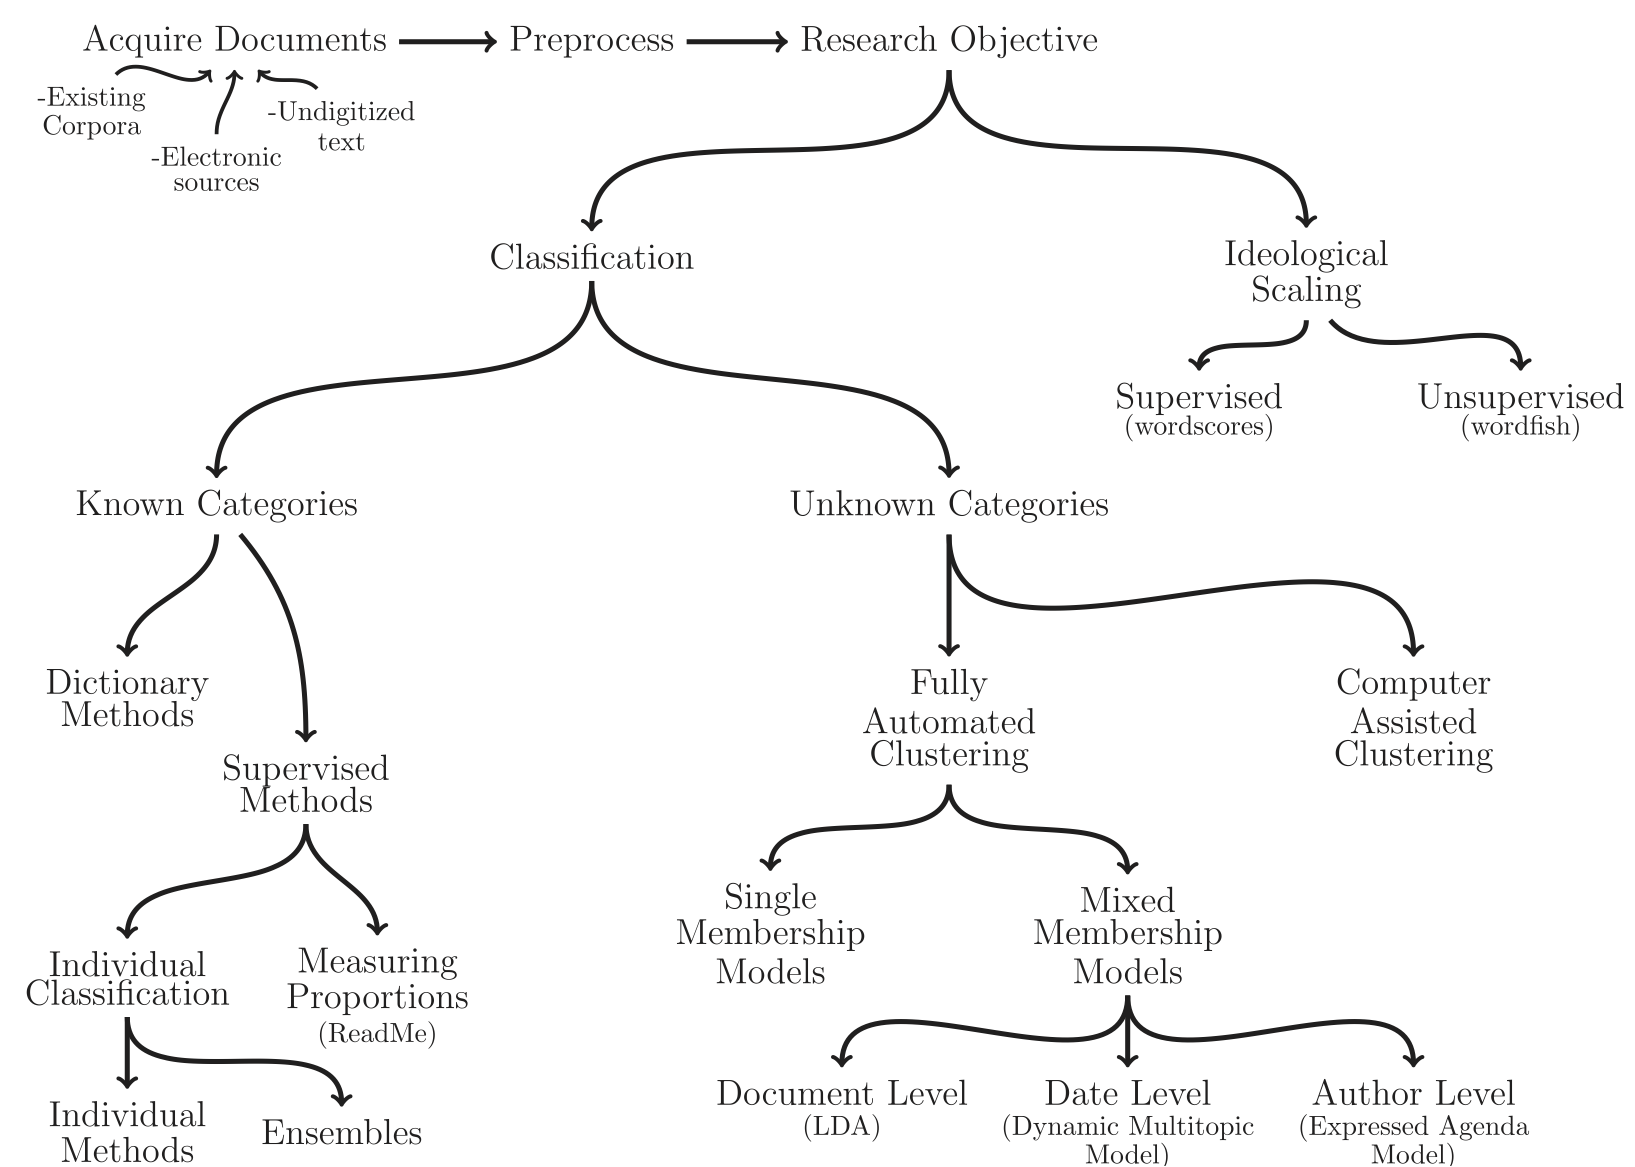
\includegraphics[width=0.7\textwidth]{../Figures/grimmer.png}
 \end{frame}



\begin{frame}{Some key concepts}
\begin{itemize}[<+->]
\item (text) corpus: a large and structured set of texts for analysis
\item Document: each of the units of the corpus (e.g. a FB post)
\item Types: for our purposes, a unique word
\item Tokens: any word--so token count is total number of words
\item For example, Doc1: ``A corpus is a set of documents'' and Doc2: ``This is the 2nd document in the corpus''.
\item This would be a corpus with 2 documents, where each document is a sentence. The first document has 6 types and 7 tokens. The second has 7 types and 8 tokens (we ignore punctuation for now).
 \end{itemize} 
\end{frame}


\begin{frame}{Some more basic concepts}
\begin{itemize}[<+->]
\item stems: words with suffixes removed (using set of rules)
\item lemmmas: canonical word form (the base form of a word that has the same meaning even when different suffixes or prefixes are attached)
\item be careful: lemmas $\neq$ stems (usage depends on analysis/RD)
\begin{table}[]
\begin{tabular}{llllll}
{\color[HTML]{6434FC} \textbf{word}}  & win & winning & wins & won & winner \\
{\color[HTML]{6434FC} \textbf{stem}}  & win & win     & win  & won & winner \\
{\color[HTML]{6434FC} \textbf{lemma}} & win & win     & win  & win & win   
\end{tabular}
\end{table}
\item stop words: words that are designated for exclusion from any analysis of a text (e.g. prepositions, uninformative verbs, pronounds...)
 \end{itemize} 
\end{frame}




  \maketitle


\end{document}